\chapter{Results and Evaluation}

\section{EDB Analysis}\label{edb analysis}
  A substantial part of my work was the exploitation of the EDB and the scraped epidemiological news.
  In the following, I introduce how I recovered parts of the EDB for my further analyses and how I managed to scrape a large amount of epidemiological data with a limited time profile.

\subsection{Source Determination}\label{source determination}
  Before I could train a classifier to detect relevant articles or extract meaningful key information from texts, I needed to create a labeled dataset from the EDB.
  Therefore, I needed to collect all articles that were read as part of INIG's surveillance routine.
  However, writing scripts for IR (such as scraping) can be time-consuming, so I needed to narrow down the, at that moment, 75 sources used in the EDB.

  The decision which source to extract was then made in regard to the relevance and the complexity to retrieve information from this source.
  First, I extracted all URLs from the EDB and clustered them based on their netloc (a first level domain such as www.rki.de) to rank the URLs according to their frequency (Fig. \ref{fig:netloc}) to then only focus on the most used sources.
  %
  \begin{figure}[h!]
    \centering
    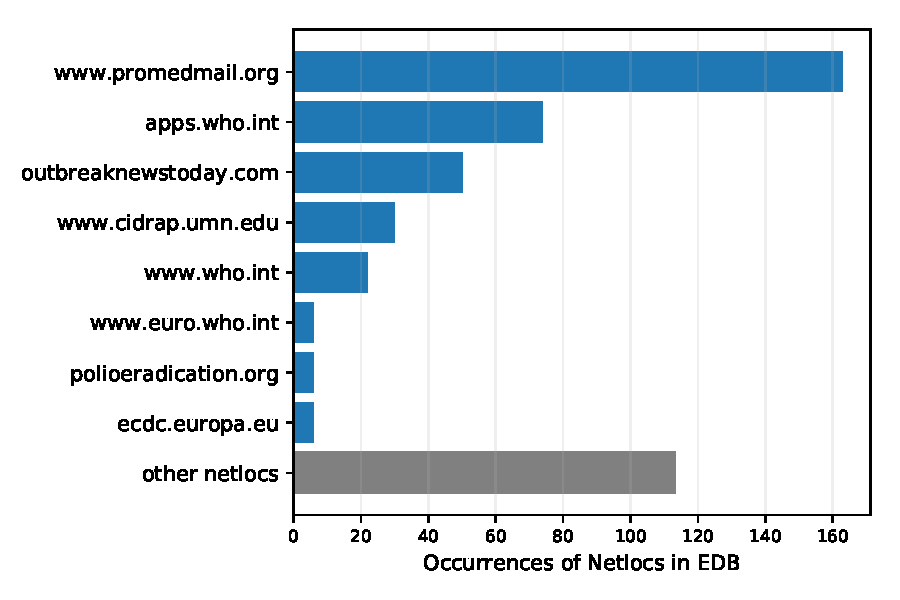
\includegraphics[scale=0.8]{netloc.pdf}
    \caption{The netloc frequency of the most used sources of the EDB. Shown in grey is the sum of EDB entries referencing the other 67 netlocs not shown in this figure.}
  \label{fig:netloc}
  \end{figure}
  %
  Then, I pinpointed those sources that are the most accessible.
  To do so, I evaluated INIG's reading checklist which includes all sources that are mandatory to observe.
  In this evaluation, I determined the data type, conducted exemplary information extractions to assess the accessibility, and evaluated the relevance of these sources by their articles (Tab. \ref{table:INIGsources}).
  %
  \begin{table}[h!]
    \centering
    \caption{An evaluation of INIG's reading checklist by source, data quality, and accessibility. The data format refers to the final data format of the epidemiological text. The data quality describes whether a source only contains information relevant for epidemiological surveillance or also research findings and ongoing projects (mixed content). The difficulty evaluation is based on exemplary IR from these sources where \textsl{easy} posed no difficulty, \textsl{intermediate} would have required additional work but was promising to function and \textsl{hard} was unsure whether it could work satisfactorily.}
    \begin{tabular}{@{}cccc@{}}
      \toprule
      \textbf{Source} & \textbf{Data Format} & \textbf{Data Quality} & \textbf{Accessibility}\\
      \midrule
      \href{http://www.cidrap.umn.edu/}{CIDRAP} & HTML & Mixed content & Intermediate \\
      \href{http://www.promedmail.org/}{ProMED Mail} & HTML & Only relevant & Easy\\
      \href{http://www.who.int/csr/don/en/}{WHO DONs} & HTML & Only relevant & Easy \\
      EIOS daily digest & Email & Only relevant & Hard \\
      \href{http://outbreaknewstoday.com/}{OutbreakNewsToday} & HTML & Mixed content & Intermediate\\
      ECDC Report & Email & Only relevant & Hard \\
      \href{http://www.afro.who.int/fr/health-topics/disease-outbreaks/outbreaks-and-other-emergencies-updates}{WHO Afro Bulletin} & PDF & Only relevant & Hard \\
      \href{http://www.eurosurveillance.org/content/eurosurveillance/browse}{EuroSurveillance} & PDF and HTML & Mixed content & Intermediate \\
      \href{http://www.who.int/wer/en/}{WHO WER} & PDF & Mixed content & Hard\\
      \href{https://ecdc.europa.eu/en/threats-and-outbreaks/reports-and-data/weekly-threats}{ECDC CDTR} & PDF & Only relevant & Intermediate \\
      \href{http://www.emro.who.int/pandemic-epidemic-diseases/information-resources/weekly-epidemiological-monitor.html}{WHO EMRO} & PDF & Mixed content & Hard \\
      \href{https://www.paho.org/hq/index.php?option=com_content&view=article&id=14044:epidemiological-alerts-archive-by-year-2018&Itemid=72203&lang=en}{WHP PAHO} & PDF & Only relevant & Intermediate\\
      \bottomrule
    \end{tabular}
    % \setlength{\tabcolsep}{1.5em}
  \label{table:INIGsources}
  \end{table}
  %
  Generally, information extraction from PDFs and Emails was more difficult.
  PDFs, unlike HTML, do not consist of a markup language where specific information can be individually extracted.
  Emails, on the other hand, were difficult to access due to privacy reasons and the information in them was usually less structured.
  The final decision was to then to scrape ProMED Mail article (163 entries in the EDB), and WHO DONs (22 entries in the EDB) indicated by \texttt{www.who.int} in Fig. \ref{fig:netloc}.
  Both are the most used HTML sources of the EDB that are also easy to scrape and only contain relevant information.
  Cidrap and OutbreakNewsToday, although being quoted more often than WHO DONs, also publish non-epidemiological articles and are harder to scrape wherefore I disregarded them.
  In sum, articles from 185 EDB entries (of 557) were scraped for the assembly of a labeled dataset using only two scrapers.
  Note, \texttt{apps.who.int} in Fig. \ref{fig:netloc}, also part of WHO, is not a WHO DON but includes several epidemiological bulletins that are published as PDFs.

\subsection{Data Quality}
  Due to the unrestrained column settings, every entry in the EDB was free text with spelling mistakes, inconsistent formatting, or left empty.
  The transferral of the EDB into a controlled vocabulary, as described in \ref{controlled vocabulary}, was a vital step since it made more data points useable.
  Tab. \ref{table:preprocessing performance} shows the performance of the data preparation.
   % for the construction of the dataset per keyword.
  \begin{table}[h!]
    \centering
    \caption{A performance measure of the transmission of the EDB to a controlled vocabulary. The table shows the number of valid entries before and after the preprocessing and the number of empty columns per keyword. The numbers refer to the whole EDB with 557 entries. The numbers in parentheses refer to the training dataset with 155 entries quoting ProMED or WHO DON articles.}
    \begin{tabular}{@{}ccccc@{}}
      \toprule
      \textbf{Keyword} & \textbf{Valid Before} & \textbf{Valid After} & \textbf{Invalid After} & \textbf{Empty Before} \\
      & \textbf{Preproc.} & \textbf{Preproc.} & \textbf{Preproc.} &\textbf{and After Preproc.} \\
      \midrule
      Date& 168 (37)& 229 (141)& 19 (7)& 309 (7) \\
      Case count& 299 (87)& 394 (105)& 18 (0)& 145 (50) \\
      Country& 355 (15) & 494 (148) & 17 (4)& 46 (3) \\
      Disease& 231 (0) & 332 (111)& 16 (16)& 209 (28) \\
      \bottomrule
    \end{tabular}
  \label{table:preprocessing performance}
  \end{table}

% \subsection{Evaluation}
  The transferral to the controlled vocabulary retrieved around 100 keywords per keyword column for the full EDB.
  Typical invalid entries for dates were dates formulated as free text like \textit{``the first two weeks in May"}.
  Another common mistake the entering of symptoms instead of diseases.
  A typical invalid country entry contained a city or region name instead of the country.
  Of 185 EDB entries referencing ProMED and WHO DON articles, 155 used valid URLs. Of the 30 invalid URLs, 8 were ProMED URLs without an article id but just (\texttt{"www.promedmail.org"}).
  The reason why only the first level domain was entered so often is the dynamical loading of articles in ProMED.
  When a user reads different articles on ProMED, the URL does not change.
  The person who wants to enter a ProMED article into the EDB needs to open the printable version of the article in order to see the unique URL of this article.
  The other URLs were correctly written but referred to articles that were not available anymore which happens when articles are withdrawn.

  % With only two scrapers and the preprocessing of the EDB entries, I was able to use 155 of the entries of the EDB to create a labeled dataset for relevance detection by analyzing the usage frequency (Fig. \ref{fig:netloc}), accessibility, and relevance of the sources (Tab. \ref{table:INIGsources}).
  Nevertheless, the preprocessing was able to increase the number of usable data points.
  For the datasets for key information extraction, 141 EDB entries with a valid date could be retrieved and 105 entries with a valid count.
  For the testing of the naive keyword selection (Lis. \ref{lst:mostoccure}) I additionally retrieved 148 entries with valid country names and 111 entries with a valid disease name.


\section{Key Information Extraction}
  Although EpiTator extracted only relevant entity classes, they still needed to be filtered for the key entity of this class, i.e., the one that would need to be put into the EDB.
  To do so, I used the most frequent entity of an entity class.
  For example, when Epitator finds relevant disease names the most frequent one is chosen (Lis. \ref{lst:mostoccure}).

  First, I used the naive key information extraction as a baseline.
  This worked well for the disease and country key information extraction but not for the date and count extraction.
  Thus, I trained a multinomial and Bernoulli NBC using all sentences of a text containing a specific entity class.
  The label \textsl{is key} was given to those sentences where the extracted entity matched the entity class found in the EDB for this text and \textsl{is not key} to the others.

\subsection{Results}\label{result keywords}
  Except for one occurrence of a disease that was not recognized by EpiTator, all countries and diseases were detected correctly using the naive key information extraction.
  However, this approach performed poorly for the key information extraction of count and date entities. Only 12 count entities of 105 were correctly retrieved (recall of 0.11 for the \textsl{is key} class and IBA of 0.10) following the naive approach and no date entity out of 141 (recall of 0.00 for the \textsl{is key} class and IBA of 0.00).

  The performance of both classifier for the key information extraction of count entities is shown in Tab. \ref{table:keyword_performance_counts} and for date entities in Tab. \ref{table:keyword_performance_dates}.
  %
  \begin{table}[h!]
    \ra{1.1}
    \caption{The performance evaluation of the count key information extraction. For each classifier and label, the precision (Pre.), recall (Rec.), specificity (Spec.), F1, index balanced accuracy (IBA) with $\alpha = 0.1$, and support (Sup.) is given. The recall of the \textsl{is key} class was the main objective of the classifier, and since the dataset was imbalanced, the IBA was a better measure for the overall accuracy. Blue values are the best in both category and orange values the worst.}
    \centering
    \begin{tabular}{@{}rcccccccc@{}}
      \toprule
       & \textbf{Pre.} & \textbf{Rec.} & \textbf{Spec.}
      & \textbf{F1} & \textbf{IBA}& \textbf{Sup} \\
      \midrule
      \textbf{Multinomial Naive Bayes}\\
      \textsl{is not key}& 0.91& 1.00& 0.00& 0.95& 0.00& 446 \\
      \textsl{is key}& 0.00& \textcolor{orange}{0.00}& 1.00& 0.00& 0.00& 43 \\
      Average/Total& 0.83& 0.91& 0.09& 0.87& \textcolor{orange}{0.00}& 489 \vspace{2mm}\\
      \textbf{Bernoulli Naive Bayes}\\
      \textsl{is not key}& 0.93& 0.90& 0.24& 0.91& 0.23& 447 \\
      \textsl{is key}& 0.18& \textcolor{cyan}{0.24}& 0.90& 0.21& 0.20& 42 \\
      Average/Total& 0.86& 0.84& 0.29& 0.85& \textcolor{cyan}{0.23}& 489 \vspace{2mm}\\
      \bottomrule
    \end{tabular}
  \label{table:keyword_performance_counts}
  \end{table}

  \begin{table}[h!]
    \ra{1.1}
    \caption{The performance evaluation of the date key information extraction. For each classifier and label, the precision (Pre.), recall (Rec.), specificity (Spec.), F1, index balanced accuracy (IBA) with $\alpha = 0.1$, and support (Sup.) is given. The recall of the \textsl{is key} class was the main objective of the classifier, and since the dataset was imbalanced, the IBA was a better measure for the overall accuracy. Blue values are the best in both category and orange values the worst.}
    \centering
    \begin{tabular}{@{}rcccccccc@{}}
      \toprule
       & \textbf{Pre.} & \textbf{Rec.} & \textbf{Spec.}
      & \textbf{F1} & \textbf{IBA}& \textbf{Sup} \\
      \midrule
      \textbf{Multinomial Naive Bayes}\\
      \textsl{is not key}& 0.67& 1.00& 0.00& 0.80& 0.00& 26 \\
      \textsl{is key}& 0.00& \textcolor{orange}{0.00}& 1.00& 0.00& 0.00& 27 \\
      Average/Total& 0.44& 0.67& 0.33& 0.53& \textcolor{orange}{0.00}& 39 \vspace{2mm}\\
      \textbf{Bernoulli Naive Bayes}\\
      \textsl{is not key}& 0.78& 0.93& 0.11& 0.85& 0.11& 30 \\
      \textsl{is key}& 0.33& \textcolor{cyan}{0.11}& 0.93& 0.17& 0.10& 9 \\
      Average/Total& 0.68& 0.74& 0.30& 0.69& \textcolor{cyan}{0.11}& 39 \vspace{2mm}\\
      \bottomrule
    \end{tabular}
  \label{table:keyword_performance_dates}
  \end{table}
  %
  Regarding the recall of the \textsl{is key} class and the IBA score, the Bernoulli NBC was performing better with a recall of 0.24 and an IBA of 0.23 for the count key information extraction. The multinomial NBC had a value of 0.00 for both these measures, and the naive approach had a recall of 0.11 and an IBA of 0.10.
  The Bernoulli NBC was also better performing than the multinomial NBC for the date key information extraction with a recall of 0.11 and an IBA 0.10 while the multinomial NBC and the naive approach had a value of 0.00 for both these measures.

  The corresponding ROC curves and their AUC values are shown in Fig. \ref{fig:roc_key}.
  %
  \begin{figure}[h!]
    \centering
    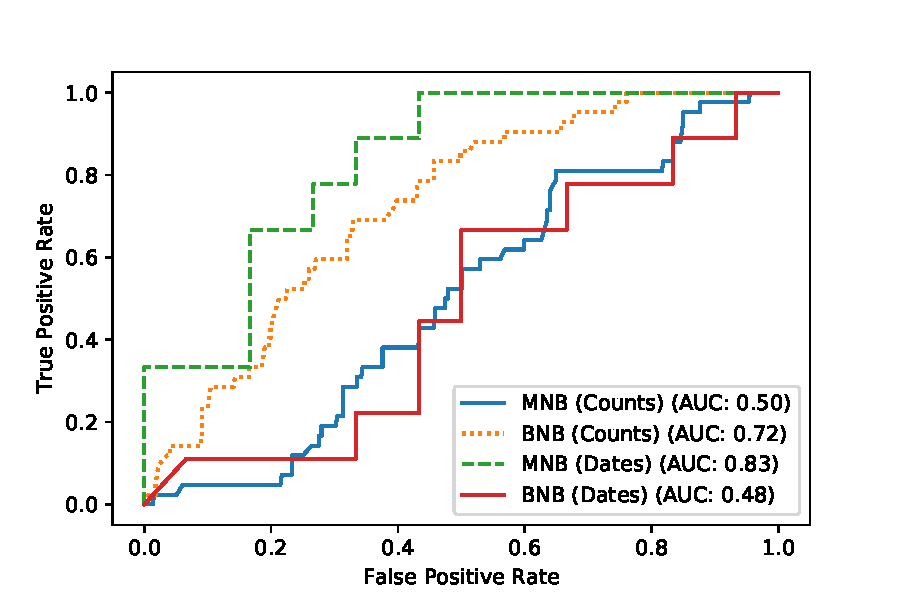
\includegraphics[scale=0.8]{roc_curves_key.pdf}
    \caption{A ROC-curve comparison of the different key information extraction classifier trained using a Multinomial naive Bayes (MNB) and Bernoulli naive Bayes (BNB) classifier with the respective value for the AUC.}
  \label{fig:roc_key}
  \end{figure}
  %
  The AUC for the count extraction was higher (0.72) for the Bernoulli NBC than the multinomial NBC (0.50).
  The AUC for the date extraction was 0.83 for the multinomial NBC and 0.48 for the Bernoulli NBC.

  Since there were strong expectations which phrases indicated the mentioning of a key entity such as \textit{``\dots confirmed cases\dots"} or \textit{``\dots cases \dots as of\dots"}, I retrieved those tokens that were strong indicators for the \textsl{is key} label (Tab. \ref{table:important_words}).

  \begin{table}[h!]
    \centering
    \caption{The most important words during the classification of the multinomial NBC to detect the key entities Counts and Dates.}
    \begin{tabular}{@{}lcc@{}}
      \toprule
      \textbf{Entity Class}& \textbf{Word} & \textbf{Positive (\%)}\\
      \midrule
      \textbf{Counts}& variant& 31.1\\
      & poultry& 27.1\\
      & Laibin& 27.1\\
      & 42-year-old& 22.2\\
      & strains.& 19.2\\
      & province.Aug& 19.2\\
      & 13For& 19.2\vspace{2mm}\\
      \textbf{Dates}
      & worm& 6.0\\
      & occurring& 5.3\\
      & Nothern& 5.3\\
      & emerging& 5.3\\
      & patients& 4.5\\
      & South& 4.1\\
      & deaths& 3.9\\
      \bottomrule
    \end{tabular}
  \label{table:important_words}
  \end{table}

\subsection{Evaluation}\label{eval_key}
  It is interesting that the multinomial NBC was by a large margin better performing in the date entity selection from sentences than the Bernoulli NBC according to the AUC (Fig. \ref{fig:roc_key}).
  This finding contradicts the former expectation that Bernoulli NBC is typically preferred in short text classifications.
  However, the contrary applies to the count entity recognition where the Bernoulli NBC indeed is better, yet with a smaller difference.
  When we regard the recall for the \textsl{is key} class and the average IBA score, then for the date and count key information extraction, the Bernoulli NBC was the better performing algorithm (Tab. \ref{table:keyword_performance_counts} and \ref{table:keyword_performance_dates}).
  In my opinion, the recall for the \textsl{relevant} class together with the IBA is critical since only correct classifications will decrease the burden for epidemiologists to enter key information into a database while the IBA gives a good measure about the overall performance of the model.
  The AUC does not seem to resemble this desired property because the multinomial NBC with the poor recall appears to be superior to the Bernoulli NBC for the date key information extraction according to the AUC.
  Thus, to maximize the usability of the key information extraction, I would prefer using the Bernoulli NBC for date and count extraction.
  It is noteworthy that both Bernoulli NBCs were better than the naive approach despite their small training data. For training the count entity extraction, 2445 labeled sentences (198 \textsl{is key} sentences) were used and for training the date entity extraction 195 labeled sentences (46 \textsl{is key} sentences).
  Surely, with more and better quality data that would result from a structured database, better results can be expected.

  Also, the words most responsible for a positive classification for an important count or date entity (Tab. \ref{table:important_words}) did not match the expectation for words like \textit{confirmed} or phrases like \textit{as of}.
  Especially the count classification is based on poor tokenization (\textit{13For}, \textit{strains.}, and \textit{province.Aug}).
  The detection of such unique (wrong) tokens in positive examples indicates a severe overfit of the classifier.
  The extracted words look more reasonable for the date classification, and the word \textit{patients} or \textit{death} appear to make sense.
  Both words could be used in a sentence where the author would also mention the date of the confirmed case numbers.
  This result suggests that the data needs to undergo better preprocessing to avoid false tokenization to achieve better results with less overfit. Note, while Tab. \ref{table:important_words} displays important features from the multinomial NBC, there is no large difference to be expected to the features of the Bernoulli NBC.
  Especially, because the Bernoulli NBC tends to overfit even more.
  The overall performance of the date and count key information extraction, however, is not good enough to be used in production. The disease and country key information extraction, on the other hand, works already well enough.

\section{Article Recommendation}
  For the detection of relevant disease outbreak articles, I used the scraped WHO DONs and ProMED Mail articles together with the EDB entries, all of the year 2018, to build a labeled dataset which consists of 155 \textsl{relevant} and 3077 \textsl{irrelevant} texts.
  Since I intended to also use word embeddings besides the bag-of-words approach to training a classifier, I visualized the word embeddings of the training data pretrained on the Wikipedia and Gigaword Corpus and self-trained embeddings using WHO DON and ProMED articles.
  Finally, I compared different classifier trained with the tf-idf transformed bag-of-word approach and document embeddings balanced with ADASYN.

\subsection{Results}
  The pretrained embeddings showed the typical clusters of similar tokens such as digits at the coordinates (-40, -90), names (-75, 25), adjectives (50, -75), and medical terms at (0, 25) (Fig. \ref{fig:t-sne}).
  The self-trained embeddings appear to cover more medical terms from the center up to the upper right corner that also seem to be clustering.
  However, it lacks other typical clusters (Fig. \ref{fig:t-sne}).
  Also, the sizable medical term cluster is not well concentrated.
  %
  \begin{figure}[h!]
    \centering
    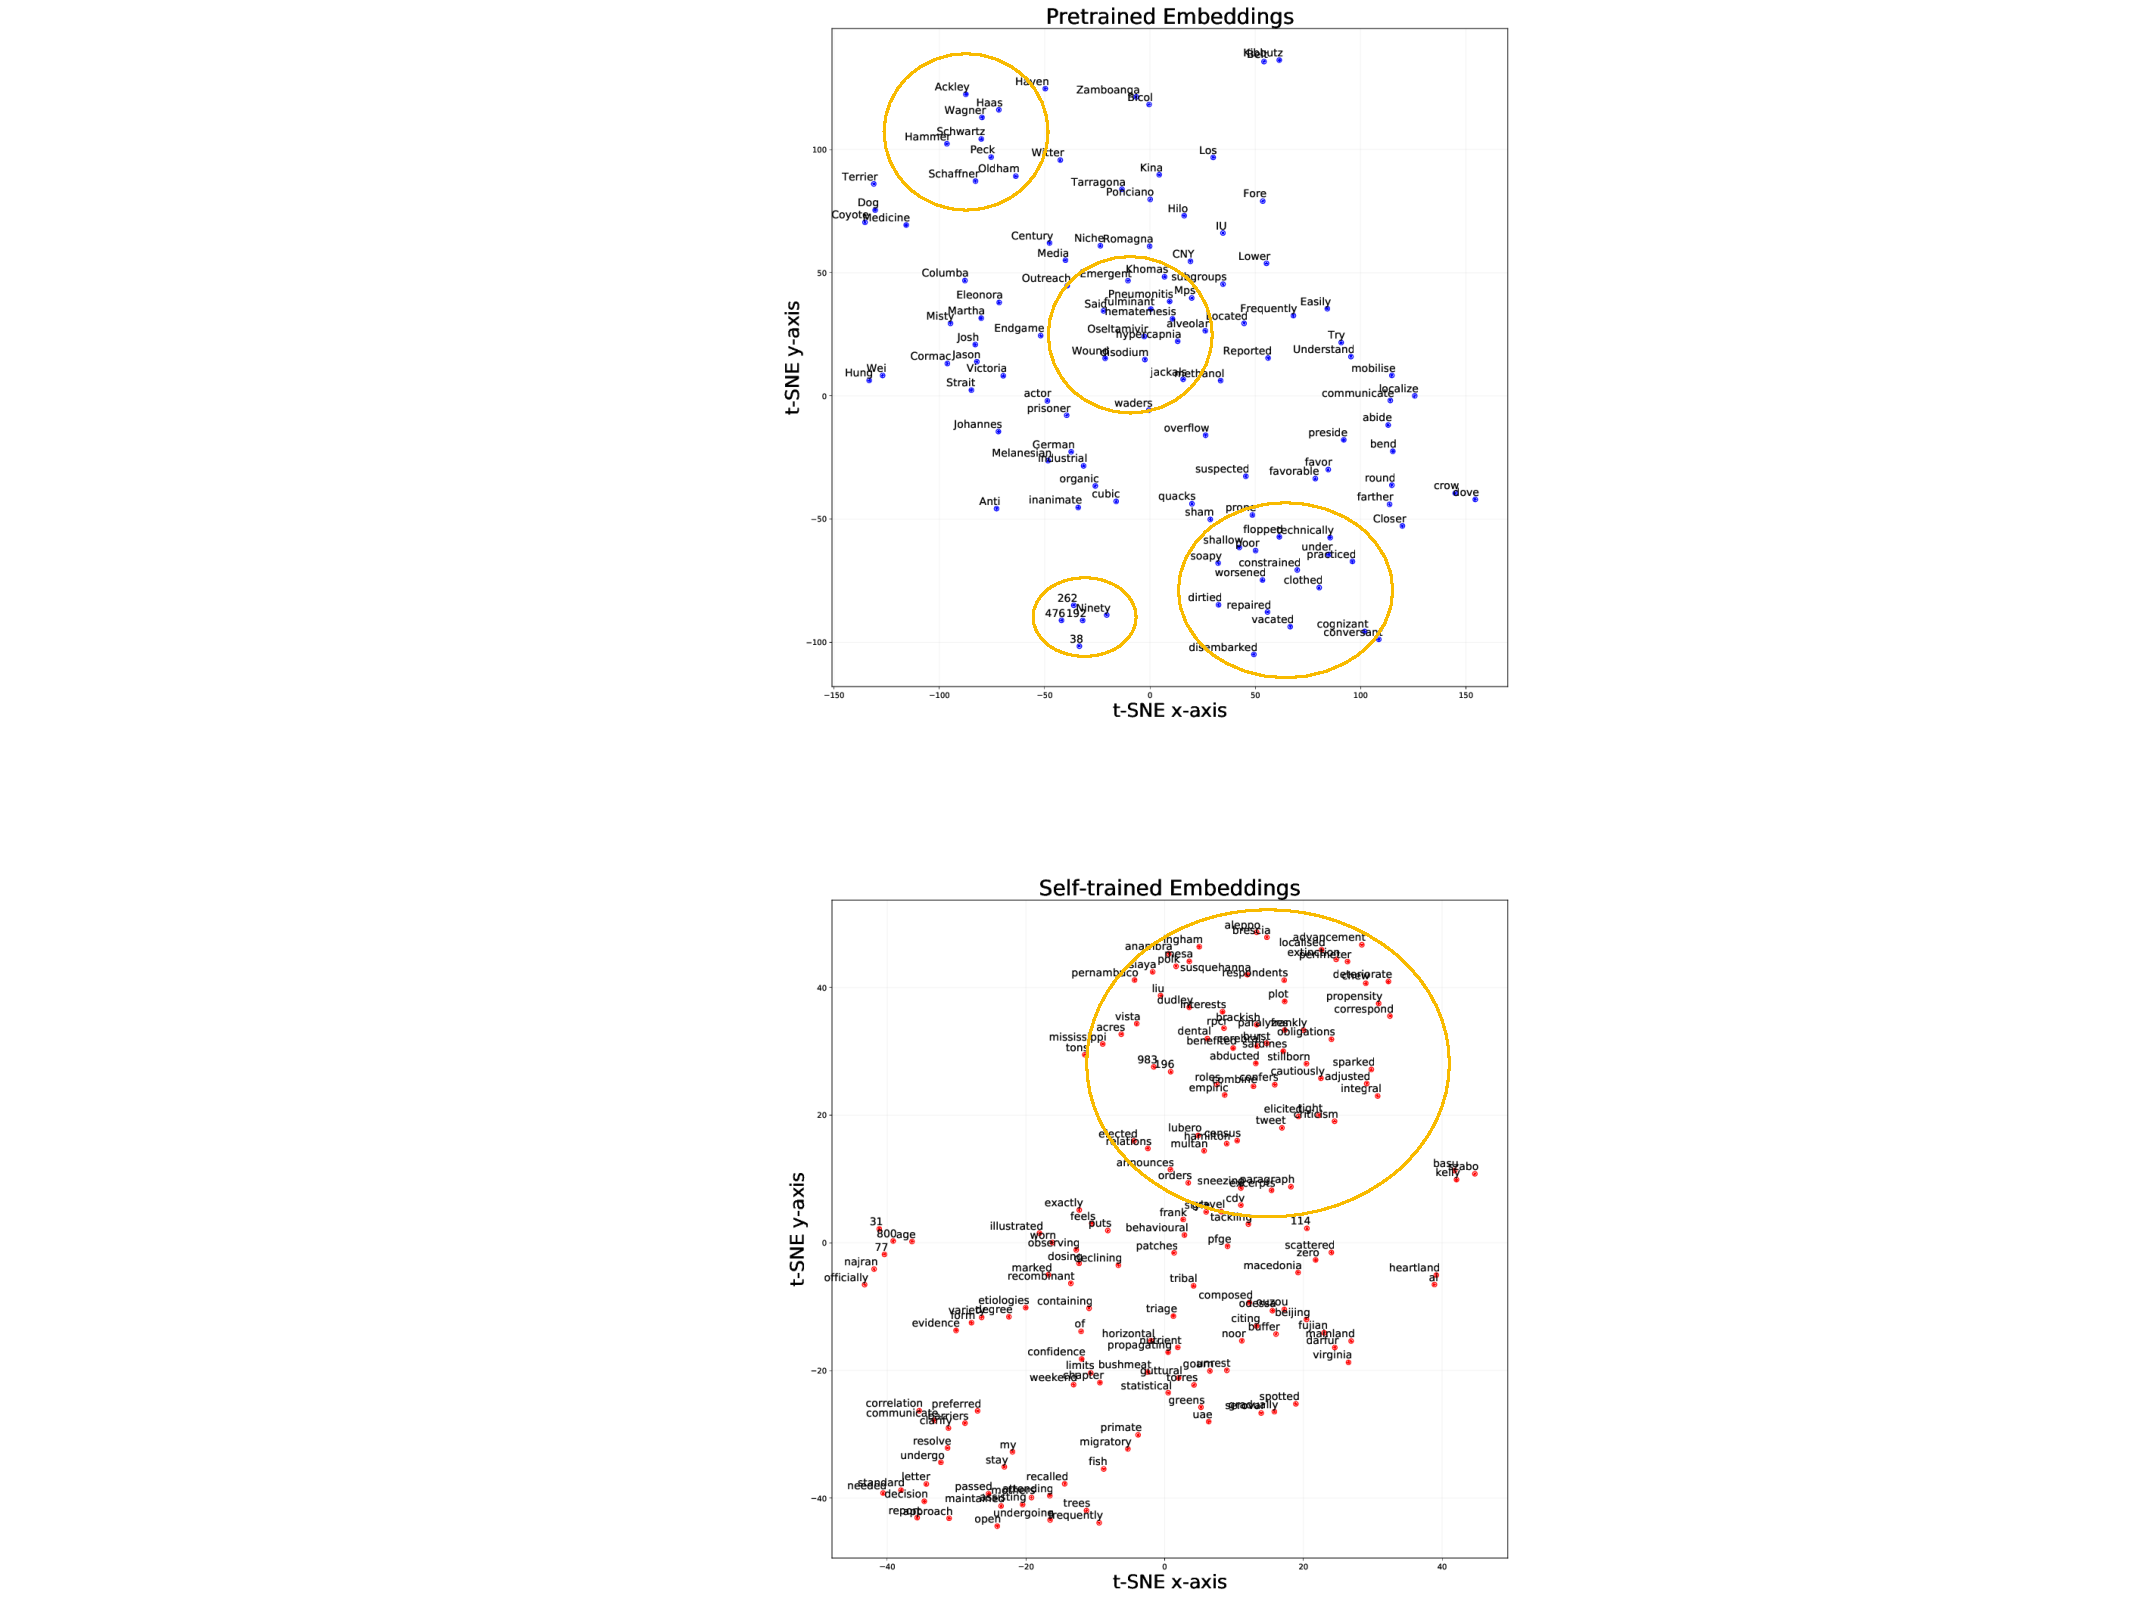
\includegraphics[scale=0.8]{t-sne-circles.pdf}
    \caption{A comparison of word embeddings applied to the training data using embeddings pretrained on the Wikipedia and Gigaword corpus (blue) and on WHO DON and ProMED articles (red) using t-SNE for dimensionality reduction. The pretrained embeddings show cluster of digits (-40, -90), names (-75, 25), adjectives (50, -75), and medical terms at (0, 25) encircled in orange. The self-trained embeddings show a neighborhood of medical terms.}
  \label{fig:t-sne}
  \end{figure}
  %

  Since the primary goal of the trained classifier is the recognition of relevant articles, the recall for the \textsl{relevant} label is essential.
  Tab. \ref{table:recommender_performance} shows that the SVM has the highest score for recall of relevant articles (0.79).
  Also, the IBA, which takes the class imbalance into account opposed to the F1 score, is the highest on average for the support vector classifier (0.47).
  The CNN is the worst performing classifier for both these measures (0.00 for both).
  The complement naive Bayes and multinomial naive Bayes classifier performed equally good (recall of 0.10 and IBA of 0.11).

  For comparison, I also plotted the ROC-curves and AUC values of all classifier (Fig. \ref{fig:roc}). The AUC value for the CNN is the highest (0.86) and for both NBC the worst (0.46).

  \begin{table}[h!]
    \ra{1.1}
    \caption{The performance evaluation of the relevance classification. For each classifier and label, the precision (Pre.), recall (Rec.), specificity (Spec.), F1, index balanced accuracy (IBA) with $\alpha = 0.1$, and support (Sup.) is given. The support vector classifier uses the radial basis function (RBF) as a kernel. Blue values are the best in their category and orange values the worst.}
    \centering
    \begin{tabular}{@{}rcccccccc@{}}
      \toprule
       & \textbf{Pre.} & \textbf{Rec.} & \textbf{Spec.}
      & \textbf{F1} & \textbf{IBA}& \textbf{Sup} \\
      \midrule
      \textbf{Multinomial Naive Bayes}\\
      \textsl{Irrelevant}& 0.96& 0.98& 0.10& 0.97& 0.11& 617 \\
      \textsl{Relevant}& 0.21& 0.10& 0.98& 0.14& 0.09& 30 \\
      Average/Total& 0.92& 0.94& 0.14& 0.93& 0.11& 647 \vspace{2mm}\\
      \textbf{Complement Naive Bayes}\\
      \textsl{Irrelevant}& 0.96& 0.98& 0,10& 0.97& 0.11& 617 \\
      \textsl{Relevant}& 0.21& 0.10& 0.98& 0.14& 0.09& 30 \\
      Average/Total& 0.92& 0.94& 0.14& 0.93& 0.11& 647 \vspace{2mm}\\
      \textbf{Logistic Regression}\\
      \textsl{Irrelevant}& 0.97& 0.67& 0.63& 0.79& 0.42& 762 \\
      \textsl{Relevant}& 0.09& 0.63& 0.67& 0.15& 0.42& 38 \\
      Average/Total& 0.93& 0.66& 0.63& 0.76& 0.42& 800 \vspace{2mm}\\
      \textbf{k-Nearest Neighbor Classifier}\\
      \textsl{Irrelevant}& 0.97& 0.77& 0.53& 0.86& 0.41& 762 \\
      \textsl{Relevant}& 0.10& 0.53& 0.77& 0.17& 0.39& 38 \\
      Average/Total& 0.93& 0.75& 0.54& 0.82& 0.41& 800 \vspace{2mm}\\
      \textbf{Support Vector Machine (RBF)}\\
      \textsl{Irrelevant}& 0.98& 0.60& 0.79& 0.74& 0.46& 762 \\
      \textsl{Relevant}& 0.09& \textcolor{cyan}{0.79}& 0.60& 0.16& 0.48& 38 \\
      Average/Total& 0.94& 0.61& 0.78& 0.72& \textcolor{cyan}{0.47}& 800 \vspace{2mm}\\
      % \textbf{Support Vector Classifier (linear)}\\
      % \textsl{Irrelevant}& 0.98& 0.65&  0.68& 0.78& 0.44& 762 \\
      % \textsl{Relevant}& 0.09& 0.68&  0.65& 0.16& 0.45& 38 \\
      % Average/Total& 0.93& 0.65& 0.68& 0.75& 0.44& 800 \vspace{2mm}\\
      \textbf{Multilayer Perceptron}\\
      \textsl{Irrelevant}& 0.97& 0.78& 0.58& 0.87& 0.46& 762 \\
      \textsl{Relevant}& 0.12& 0.58& 0.78& 0.19& 0.44& 38 \\
      Average/Total& 0.93& 0.77& 0.59& 0.83& 0.46& 800 \\
      \textbf{Convolutional Neural Network}\\
      \textsl{Irrelevant}& 0.95& 1.00& 0.00& 0.98& 0.00& 762 \\
      \textsl{Relevant}& 0.00& \textcolor{orange}{0.00}& 1.00& 0.00& 0.00& 38 \\
      Average/Total& 0.91& 0.95& 0.05& 0.93& \textcolor{orange}{0.00}& 800 \\
      \bottomrule
    \end{tabular}
  \label{table:recommender_performance}
  \end{table}

  \begin{figure}[h!]
    \centering
    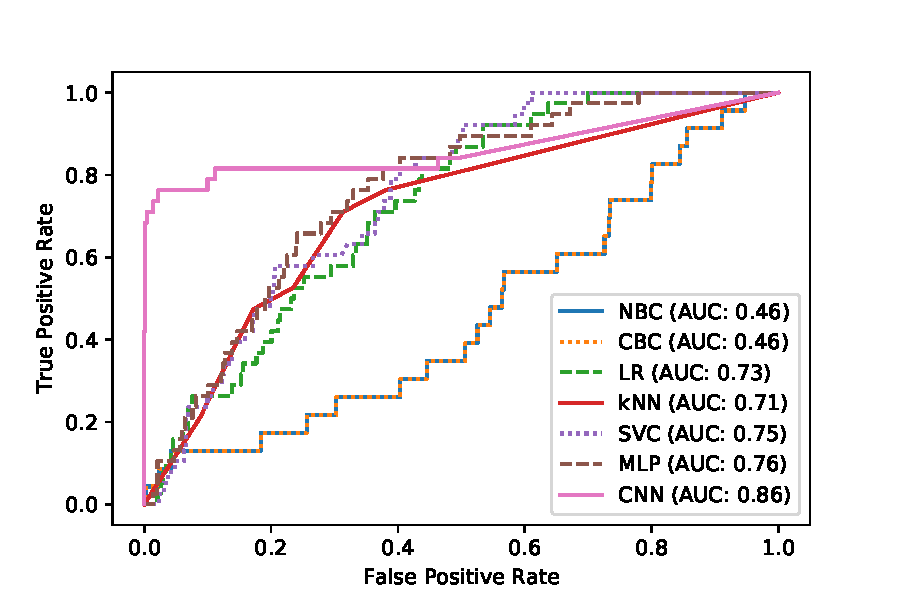
\includegraphics[scale=0.8]{roc_curves.pdf}
    \caption{A ROC-curve comparison of the different relevance classifier trained using a Multinomial naive Bayes (MNB), complement naive Bayes (CNB) classifier, logistic regression (LR), k-nearest neighbor classifier(kNN), support vector machine (SVM), multilayer perceptron (MLP) and convolutional neural network (CNN) with the respective value for the AUC. Note, the curves of the MNB and CNB overlay.}
  \label{fig:roc}
  \end{figure}

\subsection{Evaluation}\label{eval_recommend}
  The pretrained word embeddings do not cover the same amount of technical vocabulary compared to the self-trained embeddings. On the other hand, the pretrained embeddings have other semantically meaningful clusters like adjectives or names which are missing in the self-trained embeddings.
  It is likely that a more extensive corpus of epidemiological articles would show prominent technical vocabulary cluster and common word clusters at the same time which then would yield a better foundation for training classifiers.

  Against expectations, the multinomial and complement NBC had an identical performance (Tab. \ref{table:recommender_performance} and Fig. \ref{fig:roc}) although the complement NBC tackles problems occurring in imbalanced datasets specifically.
  Also, the deep learning methods worked worse concerning the imbalanced class measures and were only excelling regarding common criteria like the F1 score or the AUC value.
  It appears that the AUC value, although commonly used to measure the performance of classifier trained with imbalanced classes, does not give a good measure for the classification of \textsl{relevant} articles as the IBA or recall does since the CNN has the highest AUC score but has a recall of 0.00 for \textsl{relevant} article (Tab. \ref{table:recommender_performance}).
  A reason for the poor performance of the CNN is that it overfitted.
  Overfitting can be avoided with dropout (random removal of nodes in the network during training time to minimize highly specified nodes), regularization (e.g., L2 to punish strong weighting of nodes), and early stopping (to minimize the difference of losses between the test and validation set).
  I believe that with the aforementioned adjustments, the CNN could perform better.
  However, building a well-adjusted model was not in the scope of this thesis.

  For now, the support vector machine is preferred due to its good IBA and recall value for the \textsl{relevant} class.
  Although the relevance classification has not a strong performance, it could already aid epidemiologists.
  The model could be retrained every time articles are entered into the EDB to increase performance continuously. Until then the relevance score could just be displayed instead of using it to filter content.

\section{Web App}
  Finally, I built a web application named ``Aussinator" using Flask and Datatables to visualize a possible workflow of the keyword extraction and relevance scoring.

% \subsection{Results}
  The web app allows the user to enter an URL for evaluation.
  The output of this evaluation is the extraction of key information of this article and a relevance score  (Fig. \ref{fig:t-aussinator}).
  The app also allows a more automated workflow. The buttons \texttt{Get ProMED articles} or \texttt{Get WHO DONs} will trigger an automatic evaluation of all articles of the respective domain since the last review.
  Instead of building an automated evaluation update, this function allows the user to observe the functionality of the application better.
  Furthermore, the application has its own database that can be downloaded in different formats.
  That was an essential step at this time point since INIG was not sure how to proceed to store data.
  %
  \begin{figure}[h!]
    \centering
    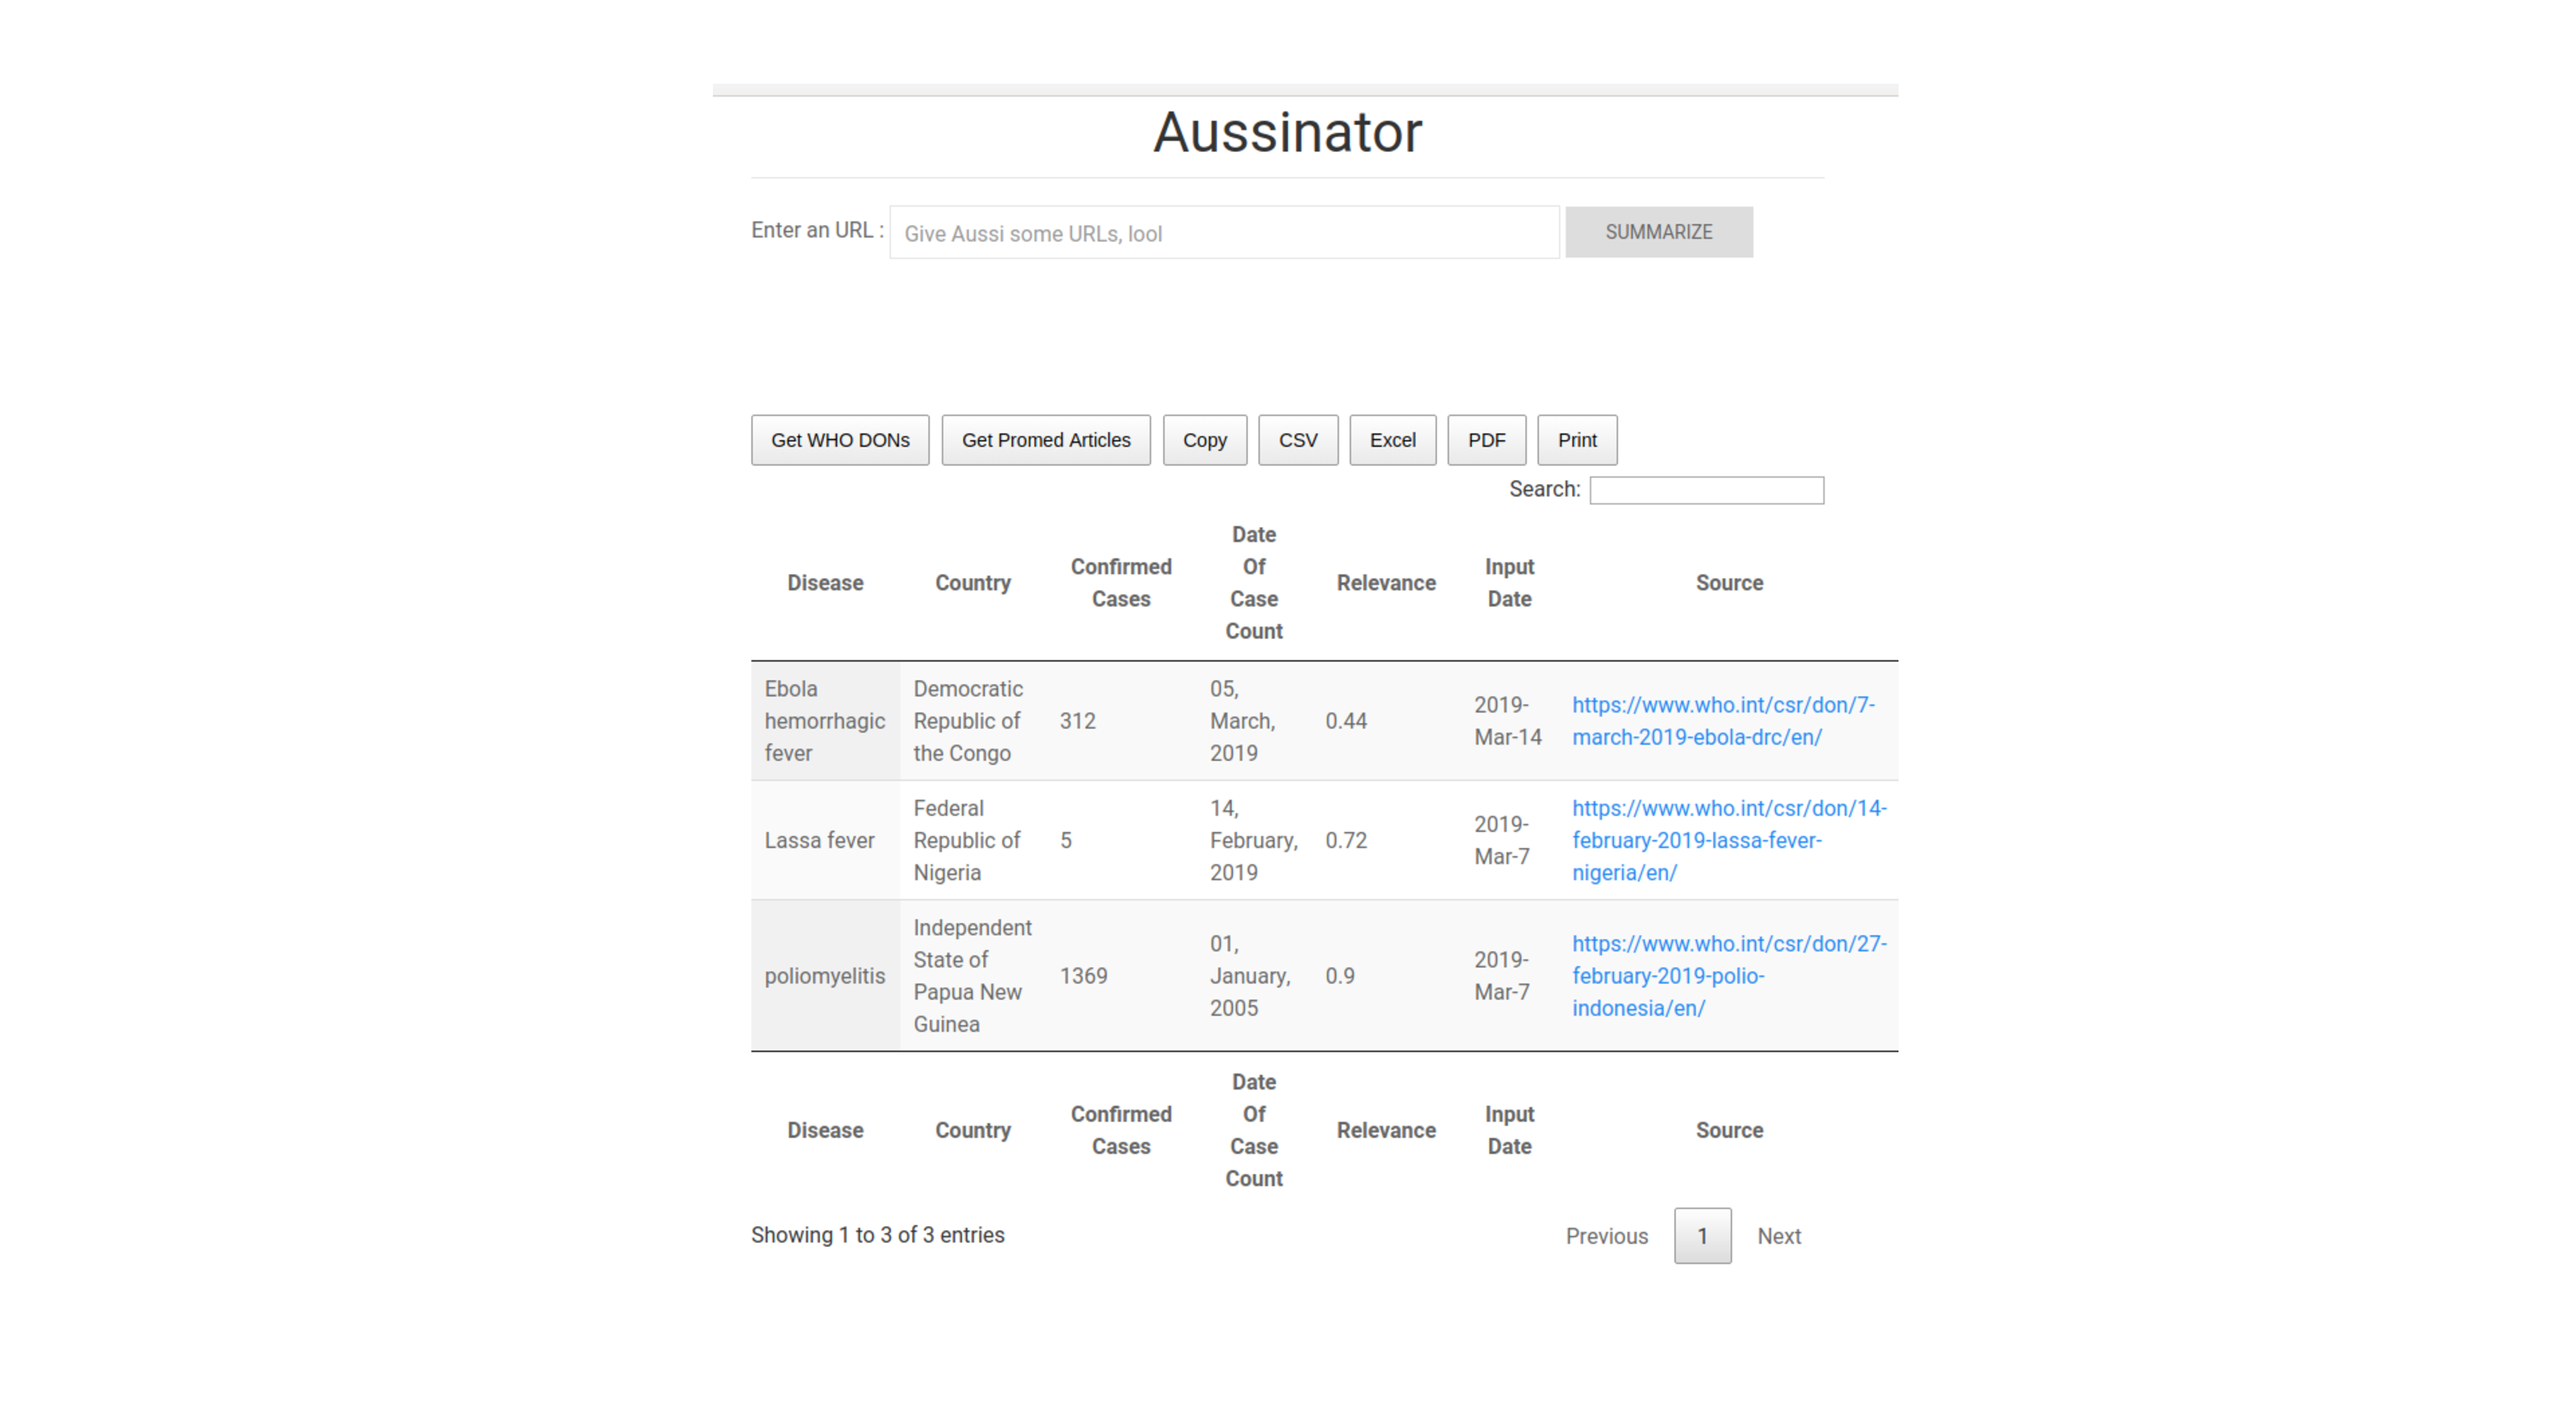
\includegraphics[scale=0.5]{aussinator.pdf}
    \caption{Aussinator, a Flask web application using the keyword extraction and relevance scoring trained as part of this thesis.}
  \label{fig:t-aussinator}
  \end{figure}
  %
% \subsection{Evaluation}

  Aussinator offers easy access to the information extraction and relevance scoring developed during this thesis. Furthermore, it provides enough freedom to the user during operation by providing a possibility to validate the output of the app.
  However, the live extraction is rather slow. The processing of one URL takes up to two seconds. This delay is particularly noticeable when extracting several articles as intended by \texttt{Get ProMED articles}.
  The preprocessing by EpiTator is the bottleneck.
  NER often is a slow process, and EpiTator looks up several entities which causes the delay.
  A solution to this would be a daemon process that regularly checks whether the sources of interest published new articles.
  If so, it would then start scraping, evaluating, and then store the key information and relevance score in the background to increase the retrieval speed for the update functions \texttt{Get ProMED articles} and \texttt{Get WHO DONs}.
